\documentclass{report}
\usepackage[utf8]{inputenc}
\usepackage[a4paper, right=2.5cm, left=2.5cm, top=2cm, bottom=2cm]{geometry}
\usepackage{graphicx}
\usepackage{media9}
\usepackage{nicefrac}
\usepackage{animate}
% \usepackage[french]{babel}

%\usepackage[default,scale=0.95]{opensans}
\usepackage{lmodern}
\usepackage[T1]{fontenc}
\usepackage{amssymb} %math
\usepackage{amsmath}
\usepackage{amsthm}
\usepackage{systeme}
\usepackage{fancyhdr}
\usepackage{hyperref}
\usepackage{float}
\usepackage{titling}
\usepackage{lipsum}
\usepackage{caption}
\usepackage{subcaption}
\usepackage{cleveref}
\usepackage{booktabs}
\usepackage{tabularx}
\usepackage[round]{natbib}
% \usepackage{subfig}

\renewcommand*\familydefault{\sfdefault} %% Only if the base font of the document is to be sans serif
\hypersetup{
    colorlinks=true,
    linkcolor=blue,
    filecolor=magenta,      
    urlcolor=cyan,
    citecolor=blue,
    pdftitle={RDFIA Report - A.Delefosse, C.Vin},
    % pdfpagemode=FullScreen,
    }
    \urlstyle{same} %\href{url}{Text}
    
    \theoremstyle{plain}% default
\newtheorem{thm}{Théorème}[section]
\newtheorem{lem}[thm]{Lemme}
\newtheorem{prop}[thm]{Proposition}
\newtheorem*{cor}{Corollaire}
%\newtheorem*{KL}{Klein’s Lemma}

\theoremstyle{definition}
\newtheorem{defn}{Définition}[section]
\newtheorem{exmp}{Exemple}[section]
% \newtheorem{xca}[exmp]{Exercise}

\theoremstyle{remark}
\newtheorem*{rem}{Remarque}
\newtheorem*{note}{Note}
%\newtheorem{case}{Case}

\title{Deep learning applications}

\author{Aymeric \textsc{Delefosse} \& Charles \textsc{Vin}}
\date{2023 -- 2024}

% Definition of \maketitle
\makeatletter         
\def\@maketitle{
    \begin{center}
        {\Huge \bfseries \sffamily \@title }\\[4ex] 
        {\Large  \@author}\\[4ex] 
        \@date\\[8ex]
        
\includegraphics[width=40cm]{../figs/sorbonne-science.pdf}
    \end{center}}
\makeatother

\fancyhead{}
\fancyhead[L]{RDFIA}\fancyhead[R]{DAC 2023 -- 2024}
\pagestyle{fancy}
\thispagestyle{plain}

\begin{document}

\begin{titlepage}
    \centering
    
    % Title
    \vspace*{\fill}
    \Huge \thetitle \par
    \vspace{2mm}
    \Large \textbf{Deep Learning Practical Work} \par
    \vspace{2mm}

    % Author
    \Large \theauthor \par
    \vspace{2mm}
    % Date
    \large \thedate \par
    
    \vfill
    
    
\includegraphics[width=0.3\textwidth]{../figs/sorbonne-science.pdf}
    
\end{titlepage}

\tableofcontents
\newpage

\section{}
\graphicspath{{figs/3b}}

\chapter{Approximate Inference in Classification}
\section{Bayesian Logistic Regression}
\subsection{Maximum-A-Posteriori Estimate}
\paragraph{1.1. Analyze the results provided by \Cref{fig:logreg_map}. Looking at $p(y=1 | x, \mathbf{w}_{\textrm{MAP}})$, what can you say about points far from train distribution?}

Approximating $p(\mathbf{w} | \mathbf{X}, \mathbf{Y})$ with a Dirac delta function is essentially akin to approximating the predictive distribution using $\mathbf{w}_{\textrm{MAP}}$, meaning $p(y=1 | x, \mathbf{w}_{\textrm{MAP}}) \approx p(y=1 | x, \mathbf{Y})$. This approximation is quite rudimentary. As depicted in \Cref{fig:logreg_map}, the model's uncertainty doesn't significantly increase far from the training data. This limitation indicates that the point-wise estimate of the parameters can only confidently assign points to their respective classes but lacks the capacity to provide nuanced uncertainty measures for points that deviate far from the training data distribution. Thus, it lacks in providing uncertainty measures for outlying points.

% The model exhibits a limitation in uncertainty estimation, remaining overconfident far from the training data, hence lacking in providing nuanced uncertainty measures for outlying points.

\begin{figure}[H]
    \centering
    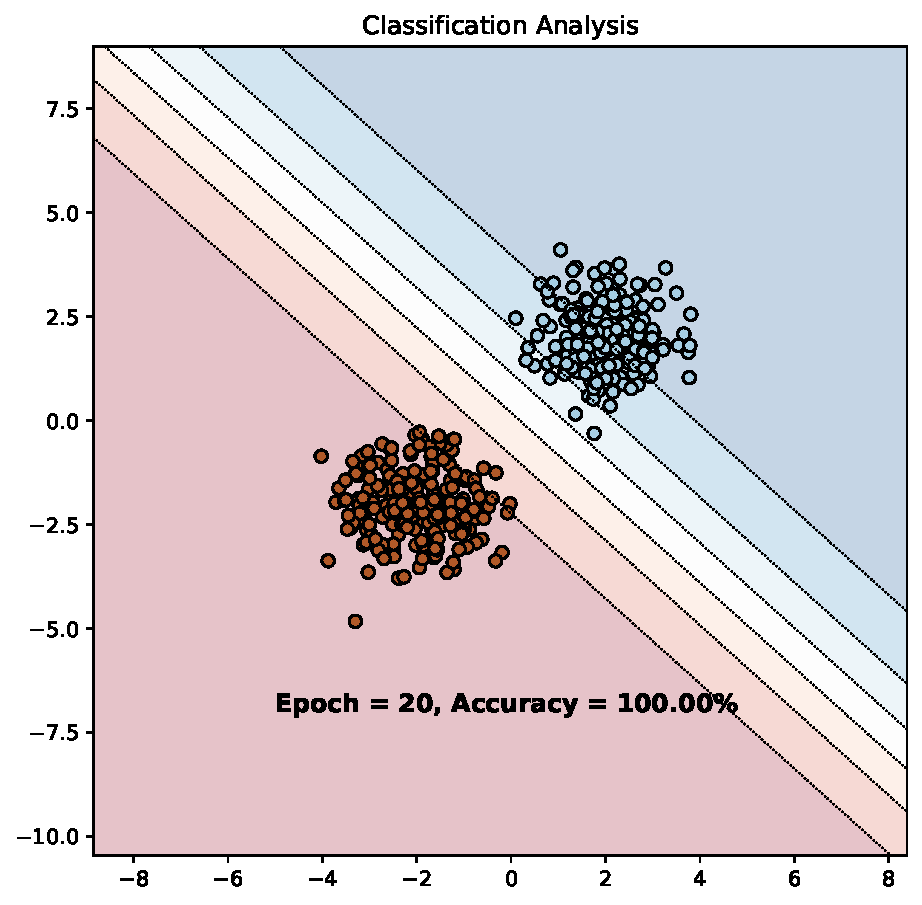
\includegraphics[width=0.45\textwidth]{logreg_map.pdf}
    \caption{Illustration of a Bayesian Logistic Regression model applied to a binary classification task with uncertainty display, with a weight decay of $5 \times 10^{-2}$. Two distinct data point clusters — blue and red — represent separate classes, while the surrounding shaded areas reflect the model's predictive uncertainty, with lighter shades indicating lower confidence.}
    \label{fig:logreg_map}
\end{figure}

\subsection{Laplace Approximation}
\paragraph{1.2. Analyze the results provided by \Cref{fig:laplace_approx}. Compared to previous MAP estimate, how does the predictive distribution behave?}

Compared to the MAP estimate, the predictive distribution in Bayesian Logistic Regression with Laplace approximation captures the uncertainty about the model parameters. While the MAP estimate provides a single point estimate of the weights ($ \mathbf{w}_{\textrm{MAP}} $), thus a single decision boundary, the Laplace approximation models the weights as a normal distribution centered around $ \mathbf{w}_{\textrm{MAP}} $ with a covariance matrix derived from the Hessian of the log posterior, which allows uncertainty in the decision boundary, as clearly displayed in \Cref{fig:laplace_approx}.

\begin{figure}[H]
    \centering
    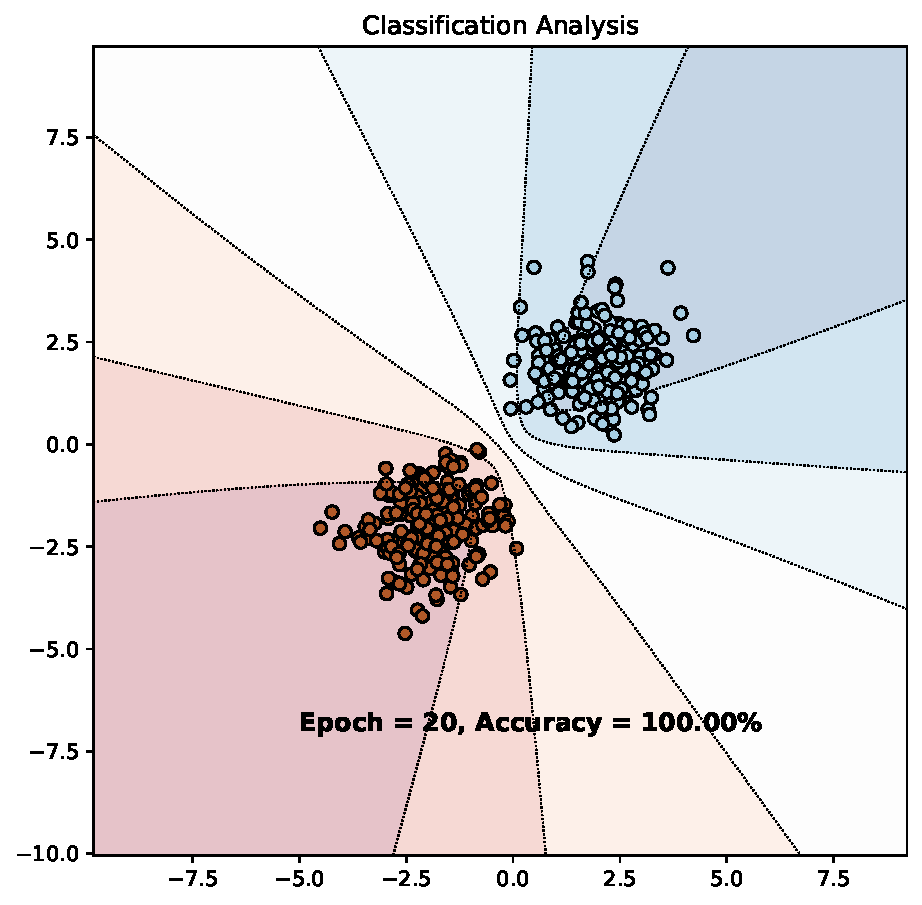
\includegraphics[width=0.45\textwidth]{laplace_approx.pdf}
    \caption{Illustration of a Bayesian Logistic Regression with Laplace approximation model applied to a binary classification task, with a weight decay of $5 \times 10^{-2}$.}
    \label{fig:laplace_approx}
\end{figure}


\paragraph{1.3. Comment the effect of the regularisation hyper-parameter  \texttt{WEIGHT\_DECAY}.}

The weight decay hyper-parameter controls the complexity of the model. It adds a penalty to the loss function for large weights, effectively encouraging the model to maintain smaller weight values. This usually help prevent overfitting by discouraging the model from relying too heavily on any single feature or combination of features.

In Bayesian terms, weight decay corresponds to the precision (inverse variance) of the prior distribution over the weights. A higher weight decay value means a tighter prior, which pulls the weights closer to zero, unless the data provides strong evidence to the contrary. This can affect the predictive distribution by potentially making it more conservative. As a result, the decision boundary may be less flexible and the model may exhibit higher uncertainty, especially in regions far from the training data. This behavior is verified in \Cref{fig:weight_decay}. When the weight decay is too high, it results in increased predictive uncertainty (wider shaded areas), whereas when it's too low, it results in high confidence (narrower shaded areas), which may not be justified for unseen data.

\begin{figure}[H]
    \centering
    \begin{subfigure}{0.45\textwidth}
        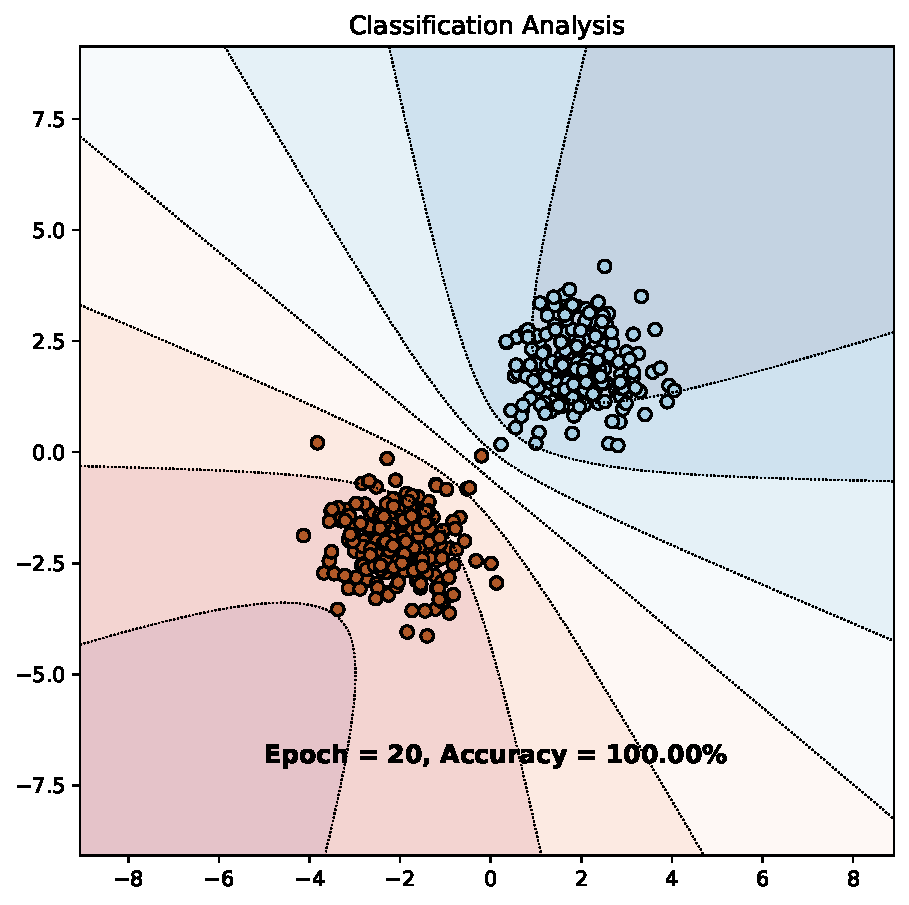
\includegraphics[width=\textwidth]{laplace_approx_0.5.pdf}
        \caption{}
        \label{subfig:weight_decay_high}
    \end{subfigure}%
    \begin{subfigure}{0.45\textwidth}
        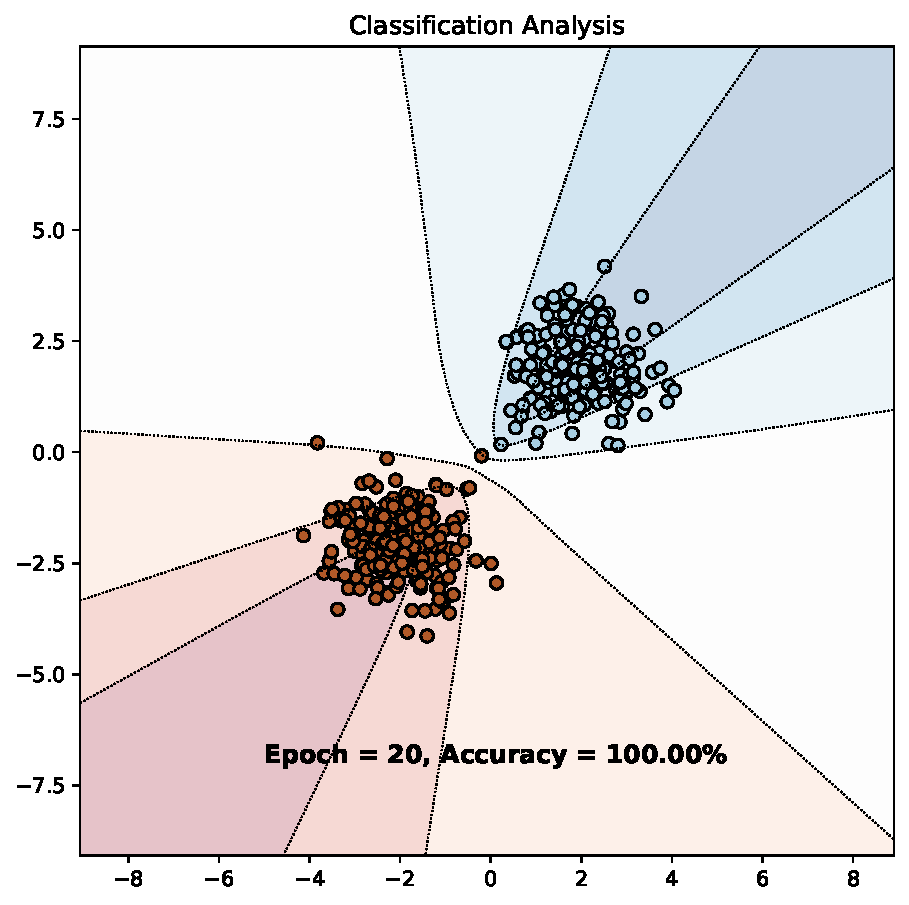
\includegraphics[width=\textwidth]{laplace_approx_5e-05.pdf}
        \caption{}
        \label{subfig:weight_decay_low}
    \end{subfigure}%
    \caption{Illustration of a Bayesian Logistic Regression with Laplace approximation model applied to a binary classification task, with a weight decay of (a) $0.5$ and (b) $5 \times 10^{-5}$.}
    \label{fig:weight_decay}
\end{figure}

\subsection{Variational Inference}
\paragraph{1.4. Comment the code of the \texttt{VariationalLogisticRegression} and \texttt{LinearVariational} classes.}

\noindent\texttt{LinearVariational} represents a single linear layer with variational inference applied. It approximates the weights and biases of the layer with distributions rather than fixed values.
\begin{itemize}
    \item The class is initialized with the variational parameters for the weights (\texttt{w\_mu}, \texttt{w\_rho}) and bias (\texttt{b\_mu}) of the layer, i.e. the parameters we want to learn. \texttt{prio\_var} represents the variance of the prior distribution ($\sigma^2_p$), to specify our prior belief about the distribution of the weights. 
    \item The \texttt{sampling} method uses the reparametrization trick to sample from the variational posterior distribution for the weights. The reparametrization trick allows the gradient of the loss function to backpropagate through the randomness of the sampling process. 
    \item The \texttt{kl\_divergence} method calculates the Kullback-Leibler divergence between the variational posterior and the prior distribution for the weights.
    \item The \texttt{forward} method defines the forward pass by sampling the weights then by computing the output of the layer using the sampled weights and the mean of the biases.
\end{itemize}

\noindent\texttt{VariationalLogisticRegression} represents a logistic regression model using variational inference:
\begin{itemize}
    \item The class is initialized with one linear variational layer used to perform the linear transformation in logistic regression.
    \item The \texttt{forward} method defines the forward pass for the logistic regression model by returning the probabilities of the positive class. 
    \item The \texttt{kl\_divergence} method simply calls the same method of the \texttt{LinearVariational} layer to obtain the KL divergence term for the model.
\end{itemize}

\paragraph{1.5. Comment the code of the training loop, especially the loss computation. Analyze the results provided by \Cref{fig:logreg_variational}. Compared to previous MAP estimate, how does the predictive distribution behave? What is the main difference between the Variational approximation and the Laplace approximation?}

The loss function calculates the Evidence Lower Bound (ELBO), which we want to maximize. In theory, we aim to maximize the likelihood of the data directly, but this is often intractable due to the integral over the weights. Therefore, we compute the Kullback-Leibler divergence between the variational distribution $q_{\theta}(w)$ and the prior distribution $p(w)$. This acts as a regularization term, encouraging the variational distribution to be similar to the prior distribution. It represents the information lost when using $q_{\theta}(w)$ to approximate $p(w)$, which we want to minimize. 

To ensure the model fits the data effectively, we compute the negative log-likelihood of the data under the model parameterized by the weights sampled from $q_{\theta}(w)$. This is done using a binary cross-entropy loss. Subsequently, we employ gradient descent (thus minimizing the negative ELBO) to update the parameters of the variational distribution to better approximate the true posterior.

Compared to a MAP estimate, the variational approach does not just find the most probable weights (as MAP does) but instead approximates the entire posterior distribution over the weights. In the variational approach, the predictive distribution captures the model's uncertainty about its predictions.

\begin{figure}[H]
    \centering
    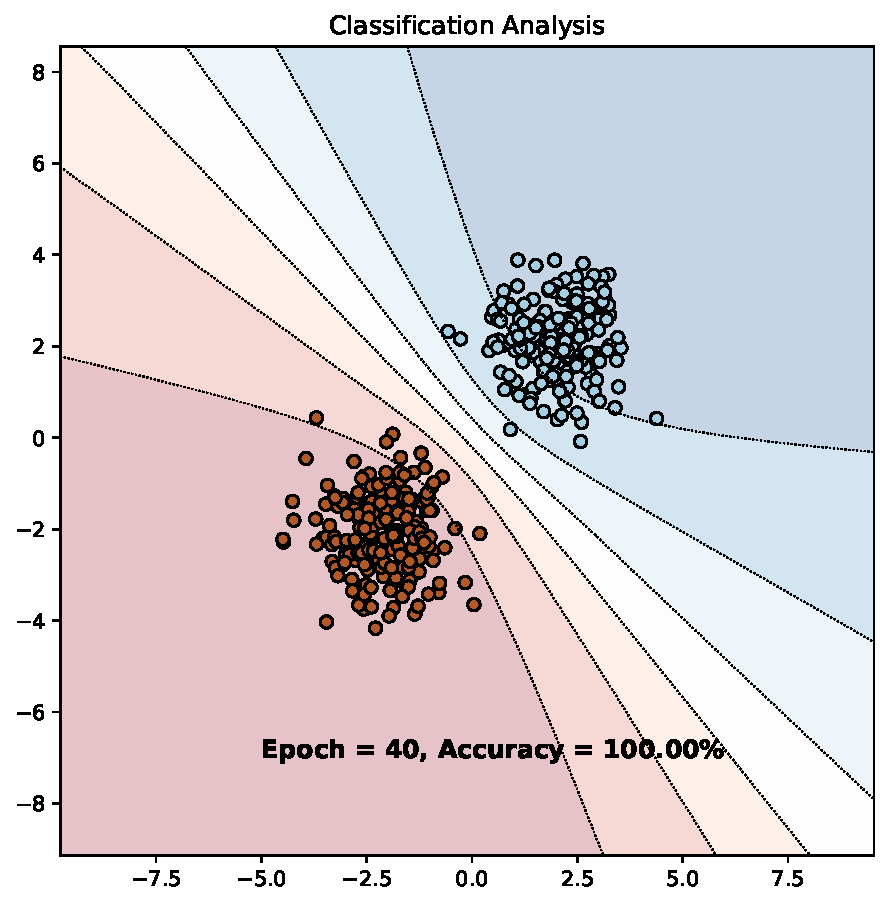
\includegraphics[width=0.45\textwidth]{logreg_variational.pdf}
    \caption{Illustration of a Variational Logistic Regression model applied to a binary classification task.}
    \label{fig:logreg_variational}
\end{figure}

\section{Bayesian Neural Networks}
\subsection{Variational Inference with Bayesian Neural Networks}
\paragraph{2.1. Analyze the results showed on \Cref{fig:mlp_variational}.}

...

\begin{figure}[H]
    \centering
    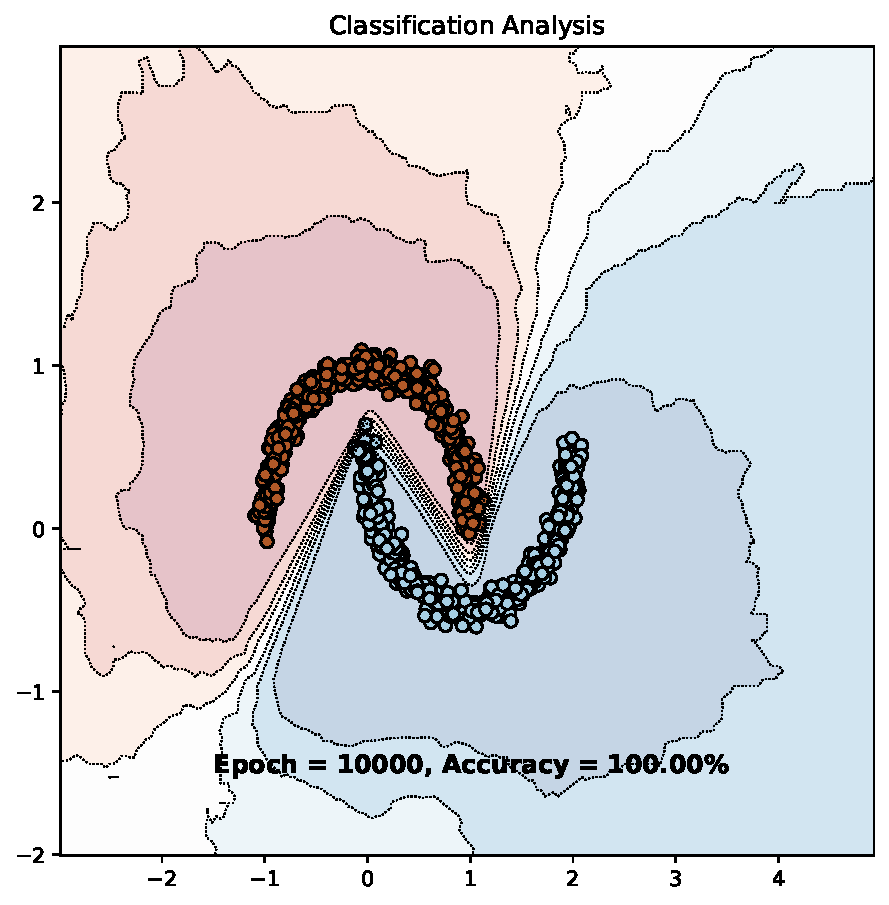
\includegraphics[width=0.45\textwidth]{mlp_variational.pdf}
    \caption{Illustration of a Bayesian Neural Network model applied to a binary classification task.}
    \label{fig:mlp_variational}
\end{figure}


\subsection{Monte Carlo Dropout}
\paragraph{2.2. Again, analyze the results showed on \Cref{fig:dropout}. What is the benefit of MC Dropout variational inference over Bayesian Logistic Regression with variational inference?}

...

\begin{figure}[H]
    \centering
    \begin{subfigure}{0.45\textwidth}
        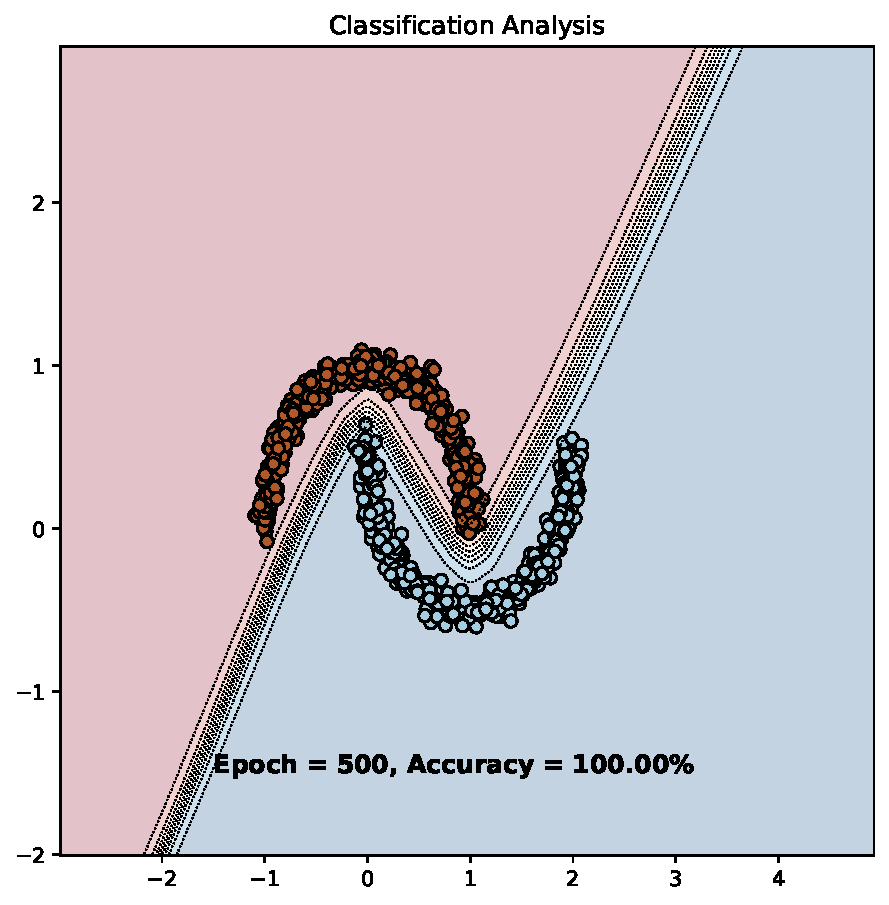
\includegraphics[width=\textwidth]{dropout.pdf}
        \caption{}
    \end{subfigure}%
    \begin{subfigure}{0.45\textwidth}
        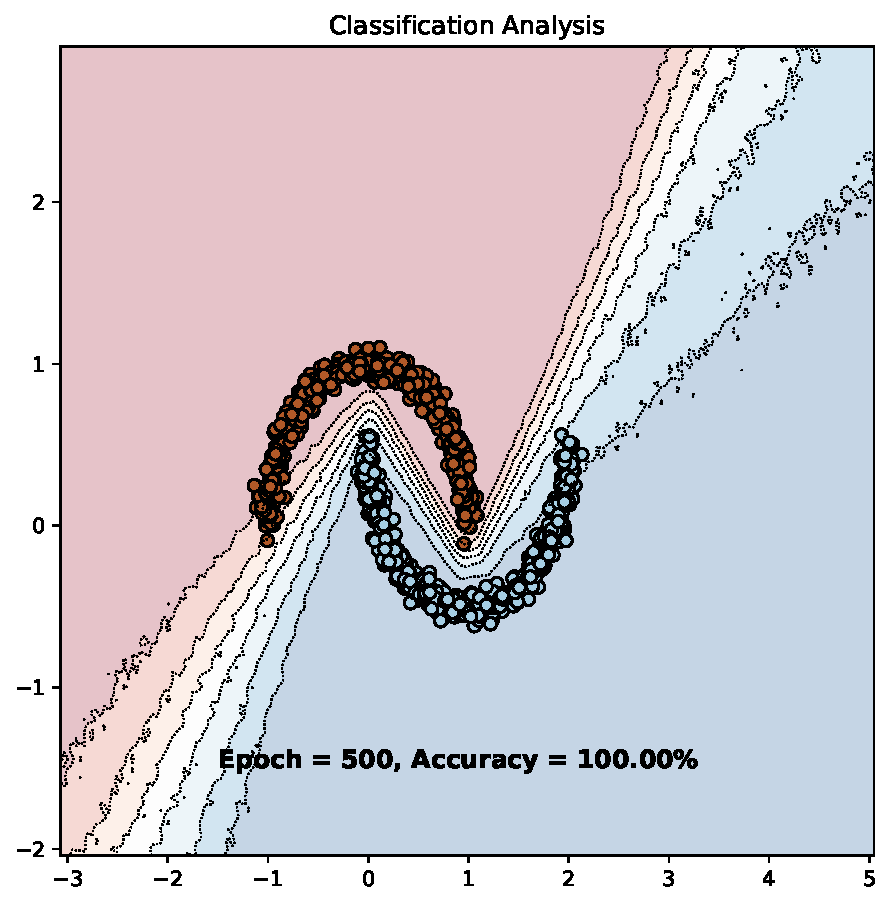
\includegraphics[width=\textwidth]{mcdropout.pdf}
        \caption{}
    \end{subfigure}%
    \caption{Illustration of a Bayesian Neural Network model applied to a binary classification task using (a) dropout and (b) Monte-Carlo dropout.}
    \label{fig:dropout}
\end{figure}

\graphicspath{{figs/3c}}

\chapter{Uncertainty Applications}
% résumé du chapitre

In this chapter, we address a significant concern in neural networks: their tendency to exhibit overconfidence in predictions. We tackle this issue by exploring uncertainty estimation techniques, notably highlighting the capabilities of Monte-Carlo Dropout variational inference, which was introduced in the previous chapter. These methods play a crucial role in mitigating overconfidence, particularly in scenarios where accurate uncertainty estimation is essential, such as failure prediction and the identification of out-of-distribution instances. This concluding chapter aims to offer a deeper comprehension and practical experience in understanding how Bayesian methods can assist us in effectively managing neural network overconfidence.

\section{Monte-Carlo Dropout on MNIST}
In this section, we focus on training a model using Monte Carlo Dropout (MC Dropout) on the MNIST dataset. Our primary aim was to identify the most uncertain samples. To do this, we used the variation ratio metric, which effectively measures epistemic uncertainty and is straightforward to calculate. For a given image, denoted as $ \mathbf{x} $, we perform $ T $ stochastic forward passes through the model and record the predicted labels. We then determine the frequency $ f^{c^\star }_\mathbf{x} $ of the most common label ($ c^\star $) across the $ T $ passes. The variation ratio for image $ \mathbf{x} $ is calculated using the formula:
\[
    \text{var-ratio}[\mathbf{x}] = 1 - \frac{f^{c^\star }_\mathbf{x}}{T}
.\]
This formula provides a quantitative measure of uncertainty for an image.

\paragraph*{1.1. What can you say about the images themselfs? How do the histograms along them helps to explain failure cases? Finally, how do probabilities distribution of random images compare to the previous top uncertain images?}

In this experiment, we used a LeNet-5 styled model with Monte-Carlo dropout variational inference. The model was train on MNIST for 20 epoch using cross-entropy in a clasical way. Then we use the model to compute the variation ratios for each test image. This permit to retrieve images by them uncertainty. That what have been done in \Cref{fig:varratio_certain,fig:varratio_certain}, they denote five measurement over the models probabilities outputs for two certain and uncertain images. To sum up the behaviour of the outputed probabilities over the $ T=100 $ stochastic forward pass, we used histograms that display four distribution.
The first columns represent the distribution of the mean of the outputed probability per class.
The second is the distribution of predicted class over the $ T $ forward passes.
Then the 3 last columns represent the distribution of the outputed probability of a particular class (the most predicted class for the 3th column, the ground truth class in the 4th column, a another different class the the 5th column).

Those histogram represent how the output probabilities vary other $ T=100 $ draw. If the model is not confident in its prediction, this will be reflected by high variation in outputed probabilities between each draw and so, histograms will be more sparce and the predicted choosen class will vary.

\Cref{fig:varratio_certain} present images caracterized as certain by the model. With our humain eye, they seem to clearly represent their denoted class. About the presented distributions, they are composed of a single peak, this mean that we approximatly draw the same value every time. The mean probabilities for the predicted class is equal to one and all other class always have a probabilitiy of zero, meaning that the model is pretty confident about it's output. 

In the other hand \Cref{fig:varratio_uncertain} present the same thing for images caracterized as uncertain by the model. Diplayed numbers seem much more ambiguous, and event with our humain eye we have diffuculties to find out which number they represent. 
Distributions are much more spreaded. What does it mean for each columns?Does it mean the same for each columns? In the following part, we will try to explain this behaviour.

For the first two columns, this only mean that many different output class neurons can be activated. To explore more this behaviour we can look at the distribution of the predicted class. As we can see, both histograms are really similar. Cela interroge sur la valeur de la probabilité lorsque la classe est prédite.

The first interpretation that come in mind is that when a class neuron is activated, around his displayed mean value, it is almost the maximum and so the choosen class. 
% j'arrive pas a expliquer, j'ai besoin d'aide en l'expliquant à quelqu'un. Je passe à la question suivante

For the third and fourth column, this mean that they can furthermore take a wide range of values (large std). Those high variation in the output probabilities and in the choosen class translate an unconfident prediction. 

\begin{figure}[H]
    \centering
    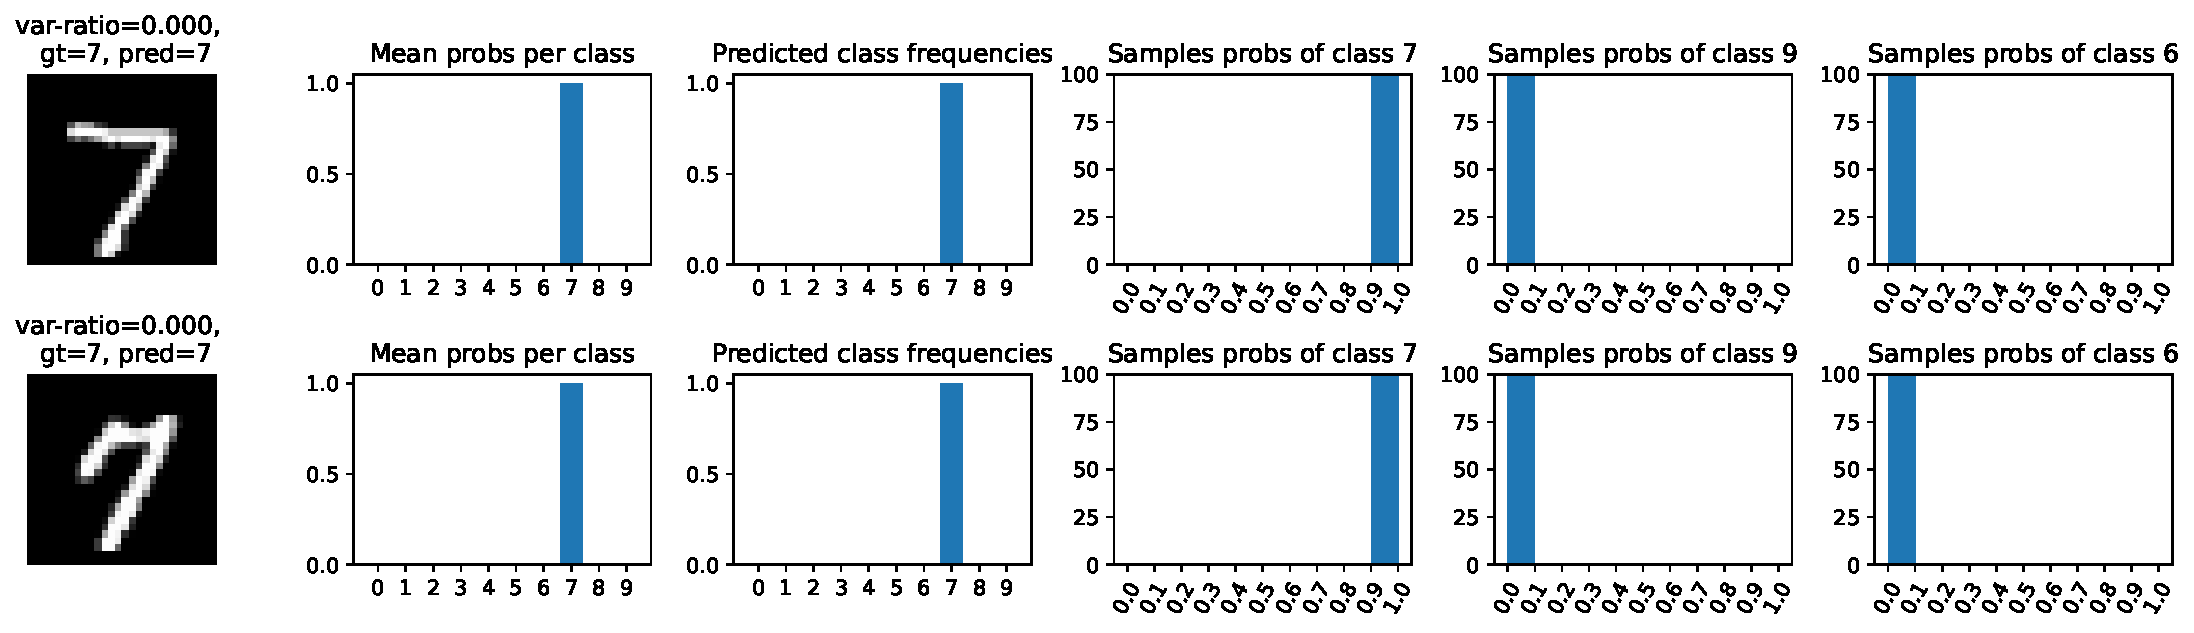
\includegraphics[width=0.95\textwidth]{var-ratio_certain_images.pdf}
    \caption{\textbf{Certain Images with Output Probability Distributions.} Images that the model classified with high certainty, featuring clear, identifiable digits. Histograms show highly concentrated distributions, with mean probabilities for the predicted class at one and other classes at zero, indicating strong model confidence in its predictions.}
    \label{fig:varratio_certain}
\end{figure}
\begin{figure}[H]
    \centering
    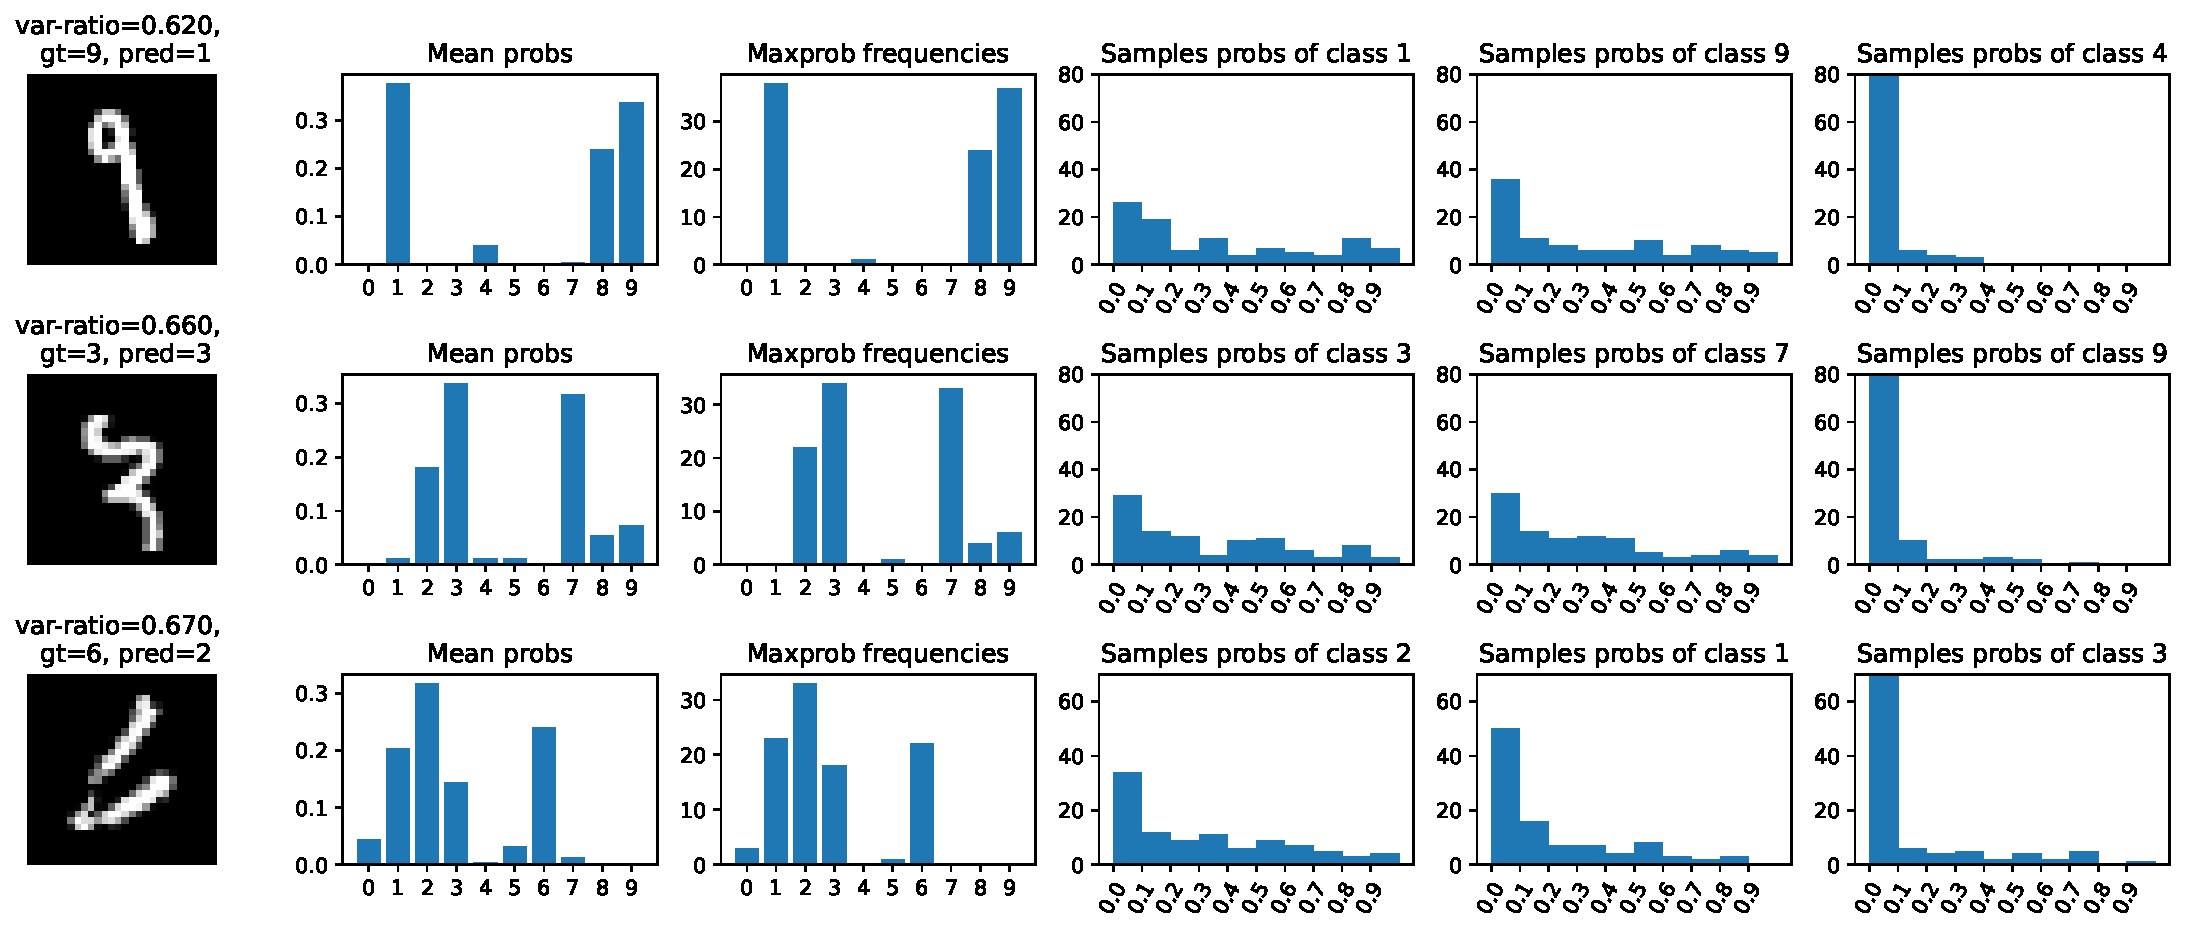
\includegraphics[width=0.95\textwidth]{var-ratio_uncertain_images.pdf}
    \caption{\textbf{Uncertain Images with Output Probability Distributions.} Ambiguous images that the model classified with uncertainty. Distributions are spread out, suggesting fluctuating confidence across different classes. The similarity between histograms of the predicted class and mean probabilities indicates that the model sometimes chooses a class with a relatively low average probability.}
    \label{fig:varratio_uncertain}
\end{figure}
\begin{figure}[hp]
    \centering
    \begin{subfigure}{0.45\textwidth}
        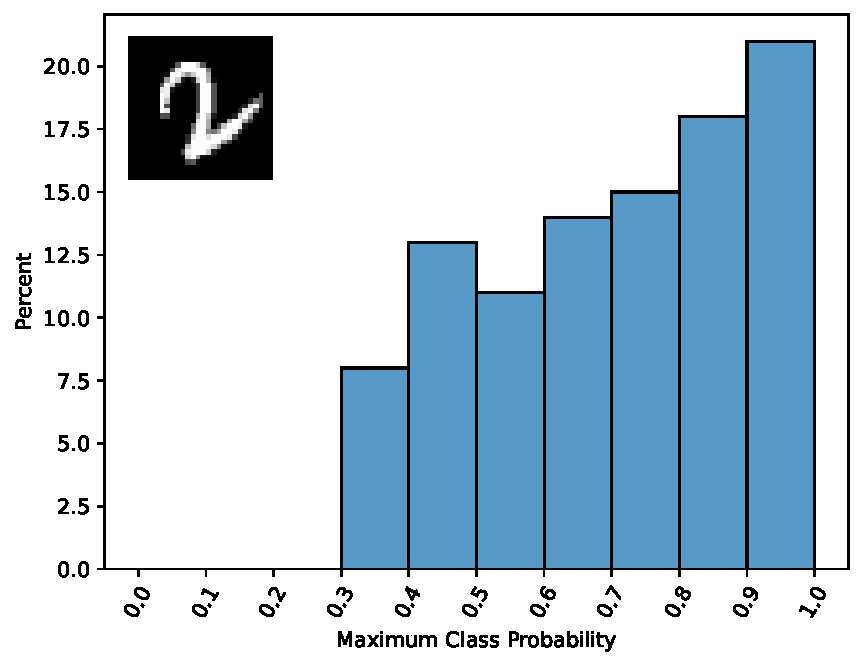
\includegraphics[width=\textwidth]{MCP_barplot.pdf}
        \caption{}
        \label{fig:MCP:barplot}
    \end{subfigure}%
    \begin{subfigure}{0.45\textwidth}
        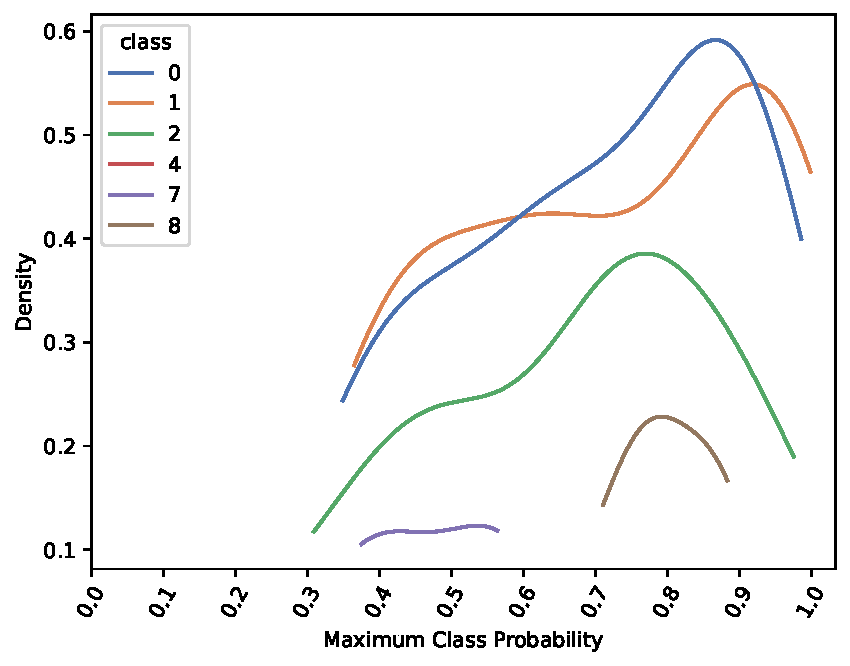
\includegraphics[width=\textwidth]{MCP_kdeplot.pdf}
        \caption{}
        \label{fig:MCP:kdeplot}
    \end{subfigure}%
    \caption{\textbf{(a) Maximum Class Probability (MCP) Bar Plot.} Bar plot showcasing the Maximum Class Probability (MCP) for uncertain images. It reveals that most predictions are based on high probability, pointing to model overconfidence. However, some decisions are made at lower probabilities, suggesting inconsistency in the model's confidence level.\\\textbf{(b) Density plot of MCP in function of the class.} KDE plot illustrating the distribution of MCP for different preditected classes, indicating the model's tendency to predict certain classes with high MCP (e.g., class 8) and others with consistently low MCP (e.g., class 7), reflecting the model's varying confidence across different classes.}
    \label{fig:MCP}
\end{figure}

\section{Failure prediction}
In this section, we have conducted a comparison of various methods aimed at obtaining a reliable confidence measure for model predictions. Such a measure permit to distinguish correct and incorrect prediction. An intelligent decision system equipped with such metrics can make informed choices, including adhering to the model's prediction or, conversely, involving a human operator, activating a backup system equipped with additional sensors, or triggering an alarm. This field of application is commonly referred to as failure prediction.

During the lecture, we found that Maximum Confidence Probability (MCP) is not a great metric for failure prediction. It assigns high confidence values to both correct and erroneous predictions because modern models tend to be overconfident, resulting in overlapping distributions between successes and errors. This issue persists even when using temperature scaling calibration.

Alternatively, when the model makes a misclassification, the probability associated with the true class $y$ tends to be lower than the maximum probability, often falling to a low value. This observation leads us to consider the True Class Probability (TCP) as a suitable measure of uncertainty. However, the true class labels $y$ are not available when estimating confidence for test inputs. This motivates the development of ConfidNet, whose primary objective is to directly regress the TCP value from the input image, allowing us to obtain a reliable measure of uncertainty without access to ground truth labels.

In this practical, we implemented ConfidNet to address failure predictions and compared it to two other methods that rely solely on the model's output probabilities. The first method is MCP, and the second is the entropy of the output probabilities. For these two methods, we used the previously trained MC Dropout model to compute the output probabilities. ConfidNet was trained for 30 epochs with the previous MC Dropout model as a teacher with frozen parameters and Mean Squared Error as the loss function.

\paragraph*{2.1. Compare the precision-recall curves of each method along with their AUPR values. Why did we use AUPR metric instead of standard AUROC?}
To assess and compare these methods, we require a suitable metric. Our objective is to identify classification errors, which we consider as the positive detection class, while correct predictions serve as the negative detection class. Since our models excel at making accurate predictions, we anticipate a low occurrence of classification errors, resulting in an imbalanced setting with a significant number of true negatives.

We have opted to employ the AUPR (Area Under the Precision-Recall Curve) instead of the AUROC (Area Under the Receiver Operating Characteristic Curve) due to the latter's unsuitability for imbalanced datasets. AUROC treats both classes equally and can yield misleading results, particularly under the influence of a large number of true negatives. This may overstate the model's performance, particularly in distinguishing the minority class, which in this context comprises classification errors. Conversely, AUPR is a more suitable choice, as it prioritizes precision and recall for the minority class. Precision measures the fraction of actual positives among the positive predictions, while recall measures the proportion of correctly identified actual positives. Consequently, AUPR proves to be a more reliable metric in our situation, where the positive class (classification errors) is significantly smaller than the negative class (correct predictions).

\Cref{fig:failure_aupr} illustrates the precision-recall curves for each method, accompanied by their respective AUPR values. The results demonstrate that ConfidNet surpasses the other two methods. This superiority can be attributed to ConfidNet's training, which directly estimates the TCP value—a more dependable uncertainty measure compared to MCP and entropy, as elaborated upon in the preceding section. Notably, ConfidNet exhibits a slower decline in precision as recall increases, indicating a more balanced performance in terms of identifying true positives without a substantial rise in false positives.

For a better understanding of the lecture's confidence metrics, we aimed to compare the performance of predictive entropy and mutual information in the context of failure detection. The results are presented in \Cref{fig:failure_aupr_entropy_vs_mut_inf}. It seems that entropy outperforms mutual information as a metric for failure detection. This distinction arises from the fact that predictive entropy measures aleatoric uncertainty, while mutual information assesses epistemic uncertainty. In the specific experiment of failure detection on MNIST, it proves more advantageous to rely on and measure aleatoric uncertainty, which originates from the natural variability or randomness of the numbers in the images. This explanation underscores why entropy is a superior metric to mutual information in this particular context.

\begin{figure}[H]
    \centering
    \begin{subfigure}{0.45\textwidth}
        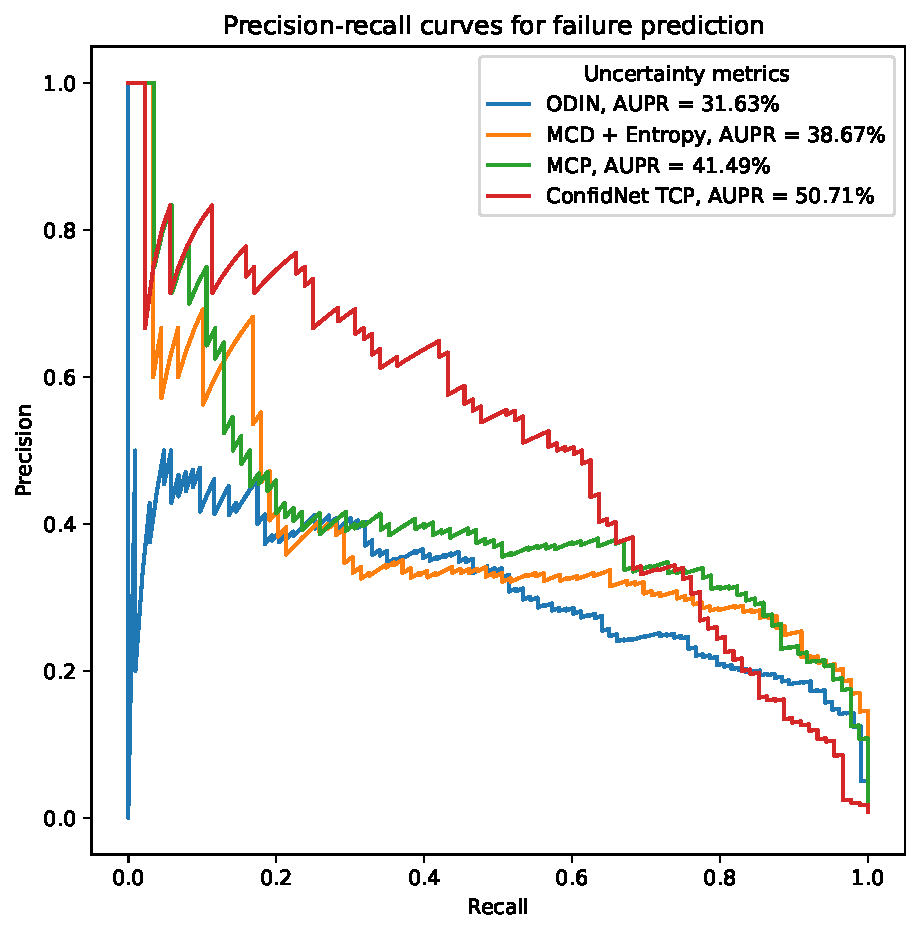
\includegraphics[width=\textwidth]{failure_aupr.pdf}
        \caption{}
        \label{fig:failure_aupr}
    \end{subfigure}%
    \begin{subfigure}{0.45\textwidth}
        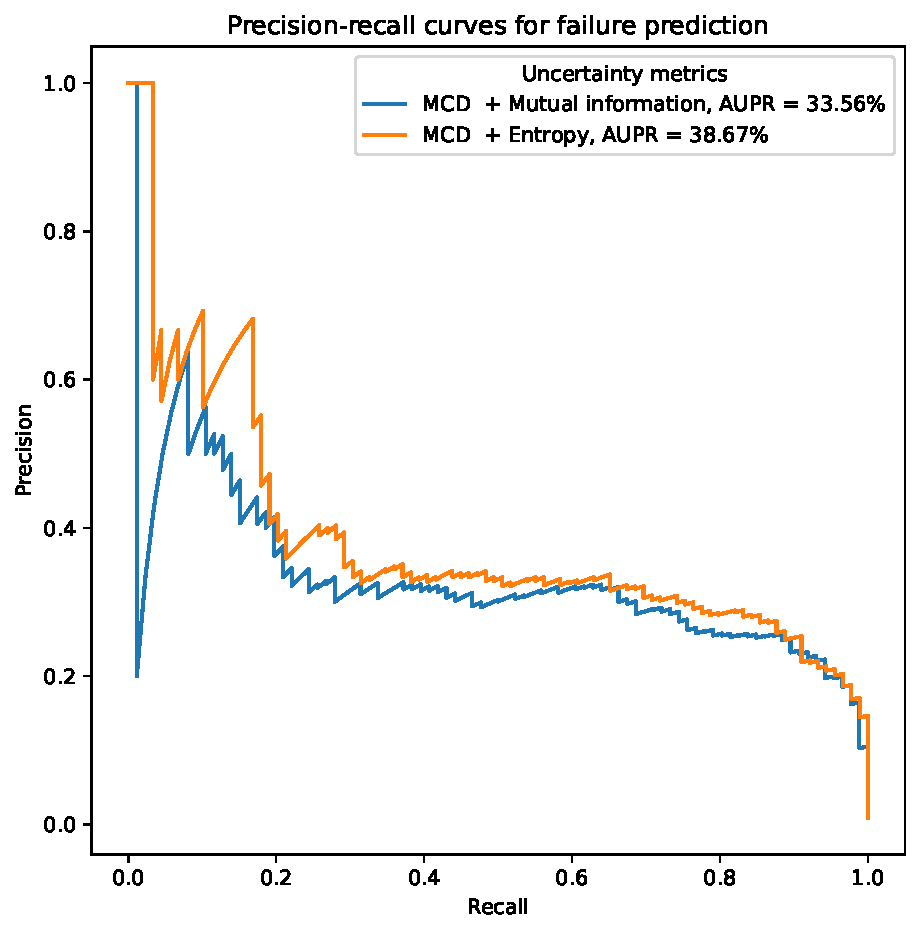
\includegraphics[width=\textwidth]{failure_aupr_entropy_vs_mut_inf.pdf}
        \caption{}
        \label{fig:failure_aupr_entropy_vs_mut_inf}
    \end{subfigure}%
    \caption{\textbf{(a) Precision-Recall Curves for Each Tested Method with AUPR Values.} The graph demonstrates ConfidNet's balanced performance in identifying true positives with fewer false positives, indicating its effectiveness in making accurate predictions with a low occurrence of classification errors.\\\textbf{(b) Performance Comparison of Predictive Entropy and Mutual Information for Failure Detection.} The graph illustrates that predictive entropy, measuring aleatoric uncertainty, outperforms mutual information, which measures epistemic uncertainty. This suggests that in scenarios with aleatoric uncertainty, like natural variability in MNIST images, entropy is a more effective metric for failure detection.}
\end{figure}

\section{Out-of-distribution detection}
In today's landscape, models are trained on millions of images, such as ImageNet, which can lead to a decrease in epistemic uncertainty. However, critical real-world applications like autonomous driving and medical imaging require the ability to detect out-of-distribution (OOD) inputs due to the stochastic nature of real-life data. In this section, we will find out what's the best methods for OOD detection. We will use the Kuzushiji-MNIST (KMNIST) dataset as out-of-distribution data for our MC dropout MNIST predictor. This dataset consists of 70,000 28x28 grayscale number images. We will evaluate the performance using precision, recall, and AUPR as metrics to compare different methods.

Specifically, in this section, we have implemented the ODIN method \citep{ODIN}, which enhances maximum softmax probabilities with temperature scaling and inverse adversarial perturbation. These techniques are employed to increase the distinction between in-distribution and out-of-distribution data.\\
Temperature scaling involves applying a simple scaling of the logit by a temperature parameter $ \nicefrac{1}{T} $ before the softmax: $ S_i(\boldsymbol{x}, T) = \frac{\exp (f_i(\boldsymbol{x}) / T)}{\sum_{j=1}^{N} \exp (f_j(\boldsymbol{x} / T))} $, where $ S_i $ represents the output probabilities, $ \boldsymbol{x} $ is the input image, $ T $ is the temperature parameter, and $ f_i $ is the logit of the $ i $-th class.\\
Inverse adversarial perturbation is used to preprocess the input $ \boldsymbol{x} $ before feeding it to the neural network. This preprocessing involves adding a small perturbation $ \epsilon $ to the input image $ \boldsymbol{x} $ such that $ \boldsymbol{x}^\prime = \boldsymbol{x} - \epsilon \cdot \text{sign}(-\nabla_{\boldsymbol{x}} \mathcal{L}(\boldsymbol{x}, y)) $, where $ \mathcal{L} $ is the cross-entropy loss function, $ y $ is the ground truth label, $ \epsilon $ is the perturbation magnitude, and $ \boldsymbol{x}^\prime $ is the perturbed image. The perturbation magnitude $ \epsilon $ is chosen to ensure the perturbed image remains correctly classified by the neural network.

\paragraph*{3.1. Compare the precision-recall curves of each OOD method along with their AUPR values. Which method perform best and why?}
\Cref{fig:OOD_aupr} displays the precision-recall curves for six uncertainty metrics (MCP, ODIN, CondifNet TCP, MC Dropout (MCD) mutual information, and MCD predictive entropy), along with their corresponding AUPR values. Given the smoothness of these curves, our analysis will primarily focus on the AUPR values.

ODIN, with its two modifications to output probabilities, performs slightly better than MCP, which aligns with expectations since ODIN builds upon MCP. However, ODIN is surprisingly surpassed by the other two methods. This outcome was not anticipated for mutual information and predictive entropy since they, like ODIN, depend on the raw output probabilities. These methods appear to benefit from the stochastic nature of MC Dropout. In fact, both methods achieved impressive AUPR scores of $98\%$, ranking as the most effective metrics for OOD detection. Despite leveraging TCP, ConfidNet trails slightly with $96\%$ AUPR. Mutual information and predictive entropy, despite their simplicity, emerge as leading metrics for OOD detection in our experiments, but at the expense of a more complex (Bayesian) network. For instance, computing the entropy score takes 18 seconds, whereas ODIN requires only 4.1 seconds.
\begin{figure}[H]
    \centering
    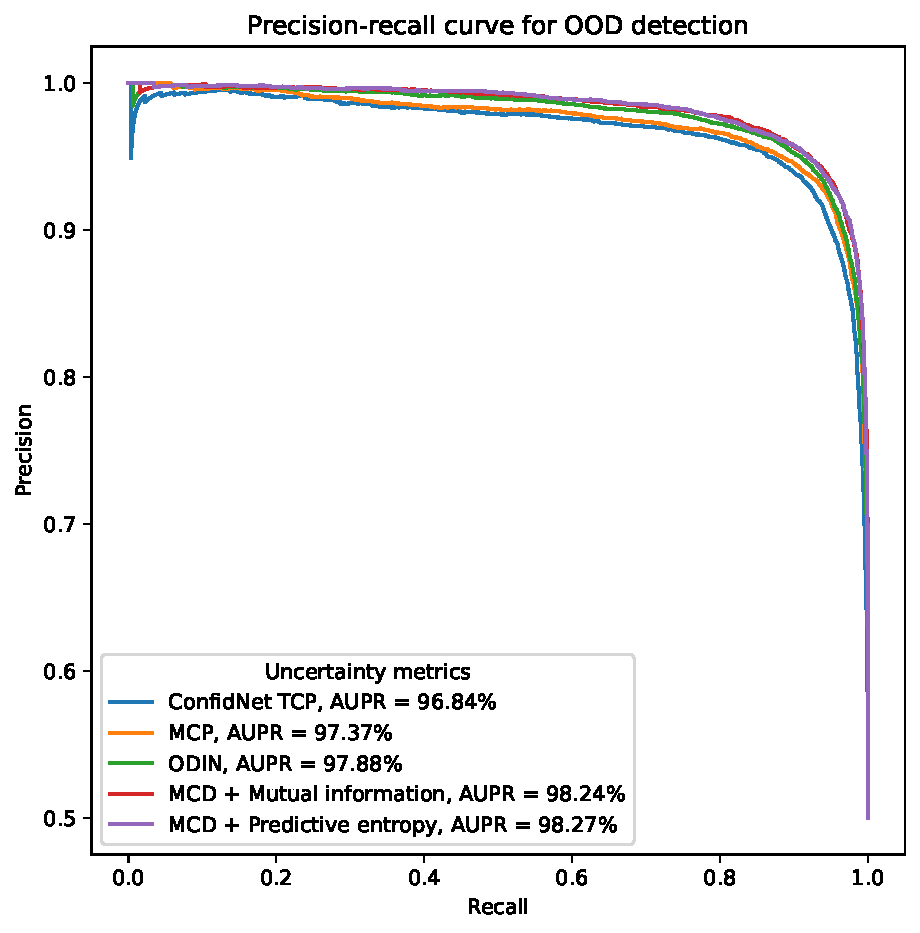
\includegraphics[width=0.45\textwidth]{OOD_aupr.pdf}
    \caption{\textbf{Precision-Recall Curves and AUPR Values for Six Uncertainty Metrics.} Precision-recall curves for six uncertainty metrics (MCP, ODIN, ConfidNet TCP, MC Dropout (MCD) mutual information, and MCD predictive entropy) with their corresponding Area Under the Precision-Recall curve (AUPR) values. MCD mutual information and predictive entropy lead with AUPR scores of $98\%$. ODIN performs slightly better than MCP but is outperformed by MCD methods, which take advantage of Bayesian networks. However, note that the performance of MCD methods comes at a computational cost.}
    \label{fig:OOD_aupr}
\end{figure}

To further investigate ODIN's techniques, we attempted to combine them with MC Dropout (averaging over 100 stochastic forward passes), predictive entropy, and mutual information. The outcomes are presented in \Cref{fig:OOD_aupr_combo}. This combination actually resulted in a slight performance decline for Entropy and Mutual Information, with a decrease of $0.3\%$ in their scores. Integrating MCD with ODIN appears to have no significant impact. 
\begin{figure}[H]
    \centering
    \begin{subfigure}{0.45\textwidth}
        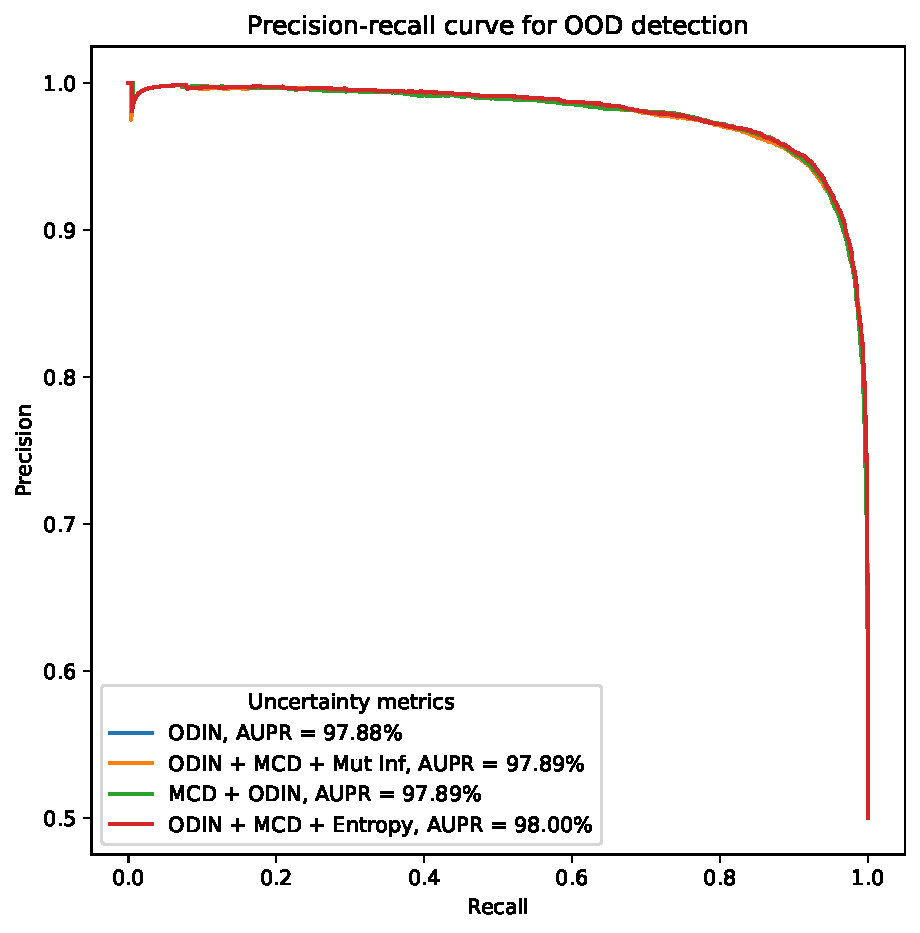
\includegraphics[width=\textwidth]{OOD_aupr_combo.pdf}
        \caption{}
        \label{fig:OOD_aupr_combo}
    \end{subfigure}%
    \begin{subfigure}{0.45\textwidth}
        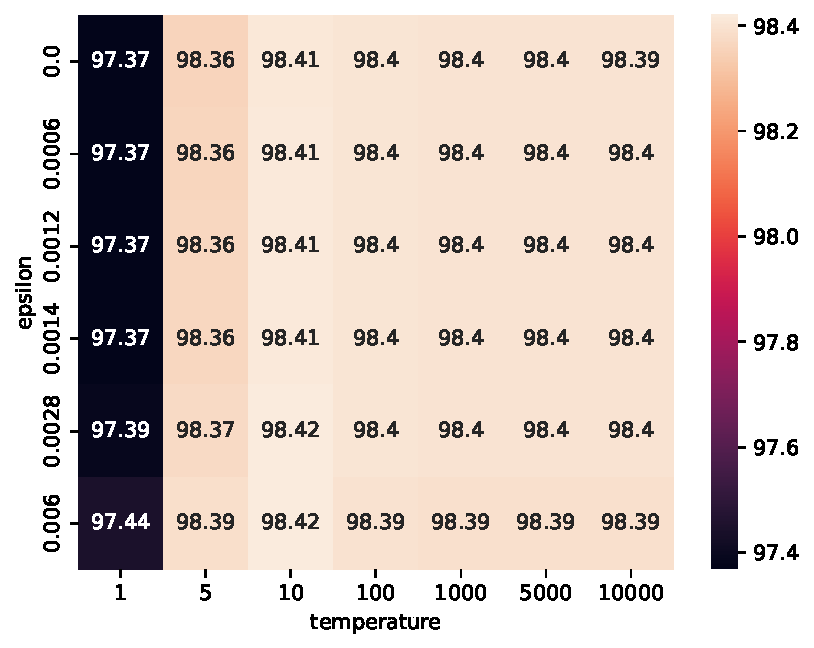
\includegraphics[width=\textwidth]{odin_grid_search.pdf}
        \caption{}
        \label{fig:odin_grid_search}
    \end{subfigure}%
    \caption{\textbf{(a) AUPR Values for Combined ODIN and MC Dropout Techniques.} Analysis of the combined impact of ODIN techniques with MC Dropout (averaging over 100 stochastic forward passes), predictive entropy, and mutual information on AUPR values. The combination slightly reduces the performance of Entropy and Mutual Information by about $0.3\%$, with no significant impact on ODIN's performance.\\\textbf{(b) Grid Search Results of ODIN's AUPR Values Relative to Hyperparameters $\epsilon$ and Temperature.} Grid search results showing the influence of ODIN's hyperparameters $\epsilon$ and temperature on its AUPR values. The best result is achieved with a temperature of 10, yielding a $98.42\%$ AUPR, surpassing MCD with entropy. Temperature scaling alone enhances AUPR by $1\%$, while perturbation has a negligible impact, suggesting temperature scaling as the more effective parameter.}
\end{figure}

Considering ODIN's persistent underperformance, we hypothesized it might be due to suboptimal hyperparameters. The code we used suggested values for $ \epsilon $ of $0.006$ and $0.0006$, but also recommended trying $ \epsilon = 0.0014 $ at the same time. Moreover, the original paper sometimes employed high temperature values, up to $10000$. This led us to conduct a grid search, the results of which, showing AUPR values in relation to $ \epsilon $ and temperature, are depicted in \Cref{fig:odin_grid_search}.

The overall influence of these parameters is noticeable, with a maximum variation of $1\%$ between the highest and lowest scores. Setting the temperature to $ 10 $ yielded the best result, achieving a $98.42\%$ AUPR, surpassing MCD with entropy which scored $98.25\%$. Setting the temperature to $ 1 $ essentially disables temperature scaling, allowing us to isolate the effect of perturbation, and vice versa for $ \epsilon = 0 $. Hence, the first cell serves as a baseline for comparison with other cells. The first line indicates that temperature scaling alone can enhance AUPR by $1.1\%$, a modest but significant improvement given the close scores. However, examining the first column reveals no discernible impact of perturbation at any $ \epsilon $ value, suggesting that combining both parameters achieves similar results to using temperature scaling alone. As the provided code uses a smaller epsilon for OOD data, we also replicated the grid search with this adjustment, which led to analogous findings.
\begin{figure}[H]
    \centering
    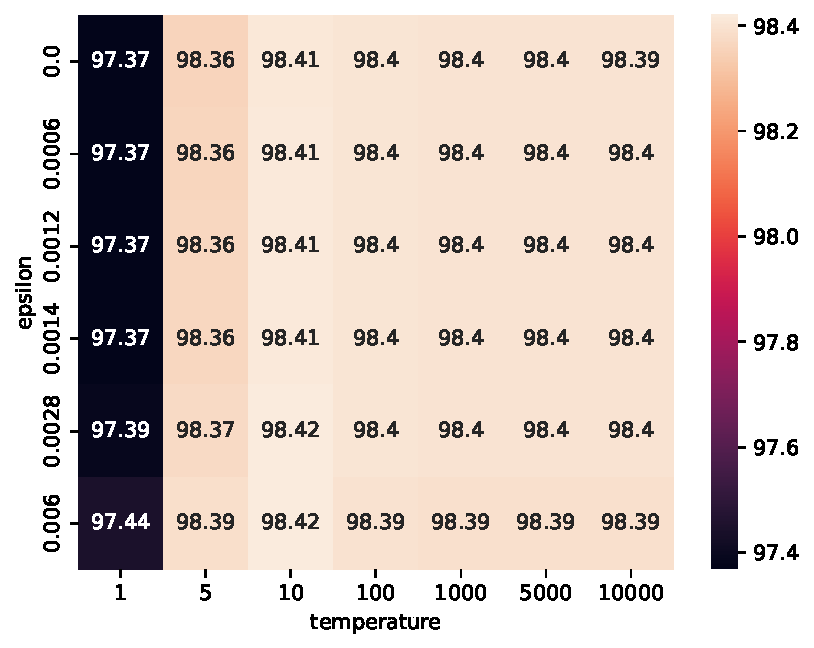
\includegraphics[width=0.45\textwidth]{odin_grid_search.pdf}
    \caption{}
    \label{fig:odin_grid_search}
\end{figure}

% \bibliographystyle{plainnat}
% \bibliography{bib}

\end{document}